\documentclass[tikz, border=5pt]{standalone}

\usepackage{tikz}
\usetikzlibrary{
    positioning,
    arrows.meta,
    shapes.geometric,
    calc
}

\begin{document}

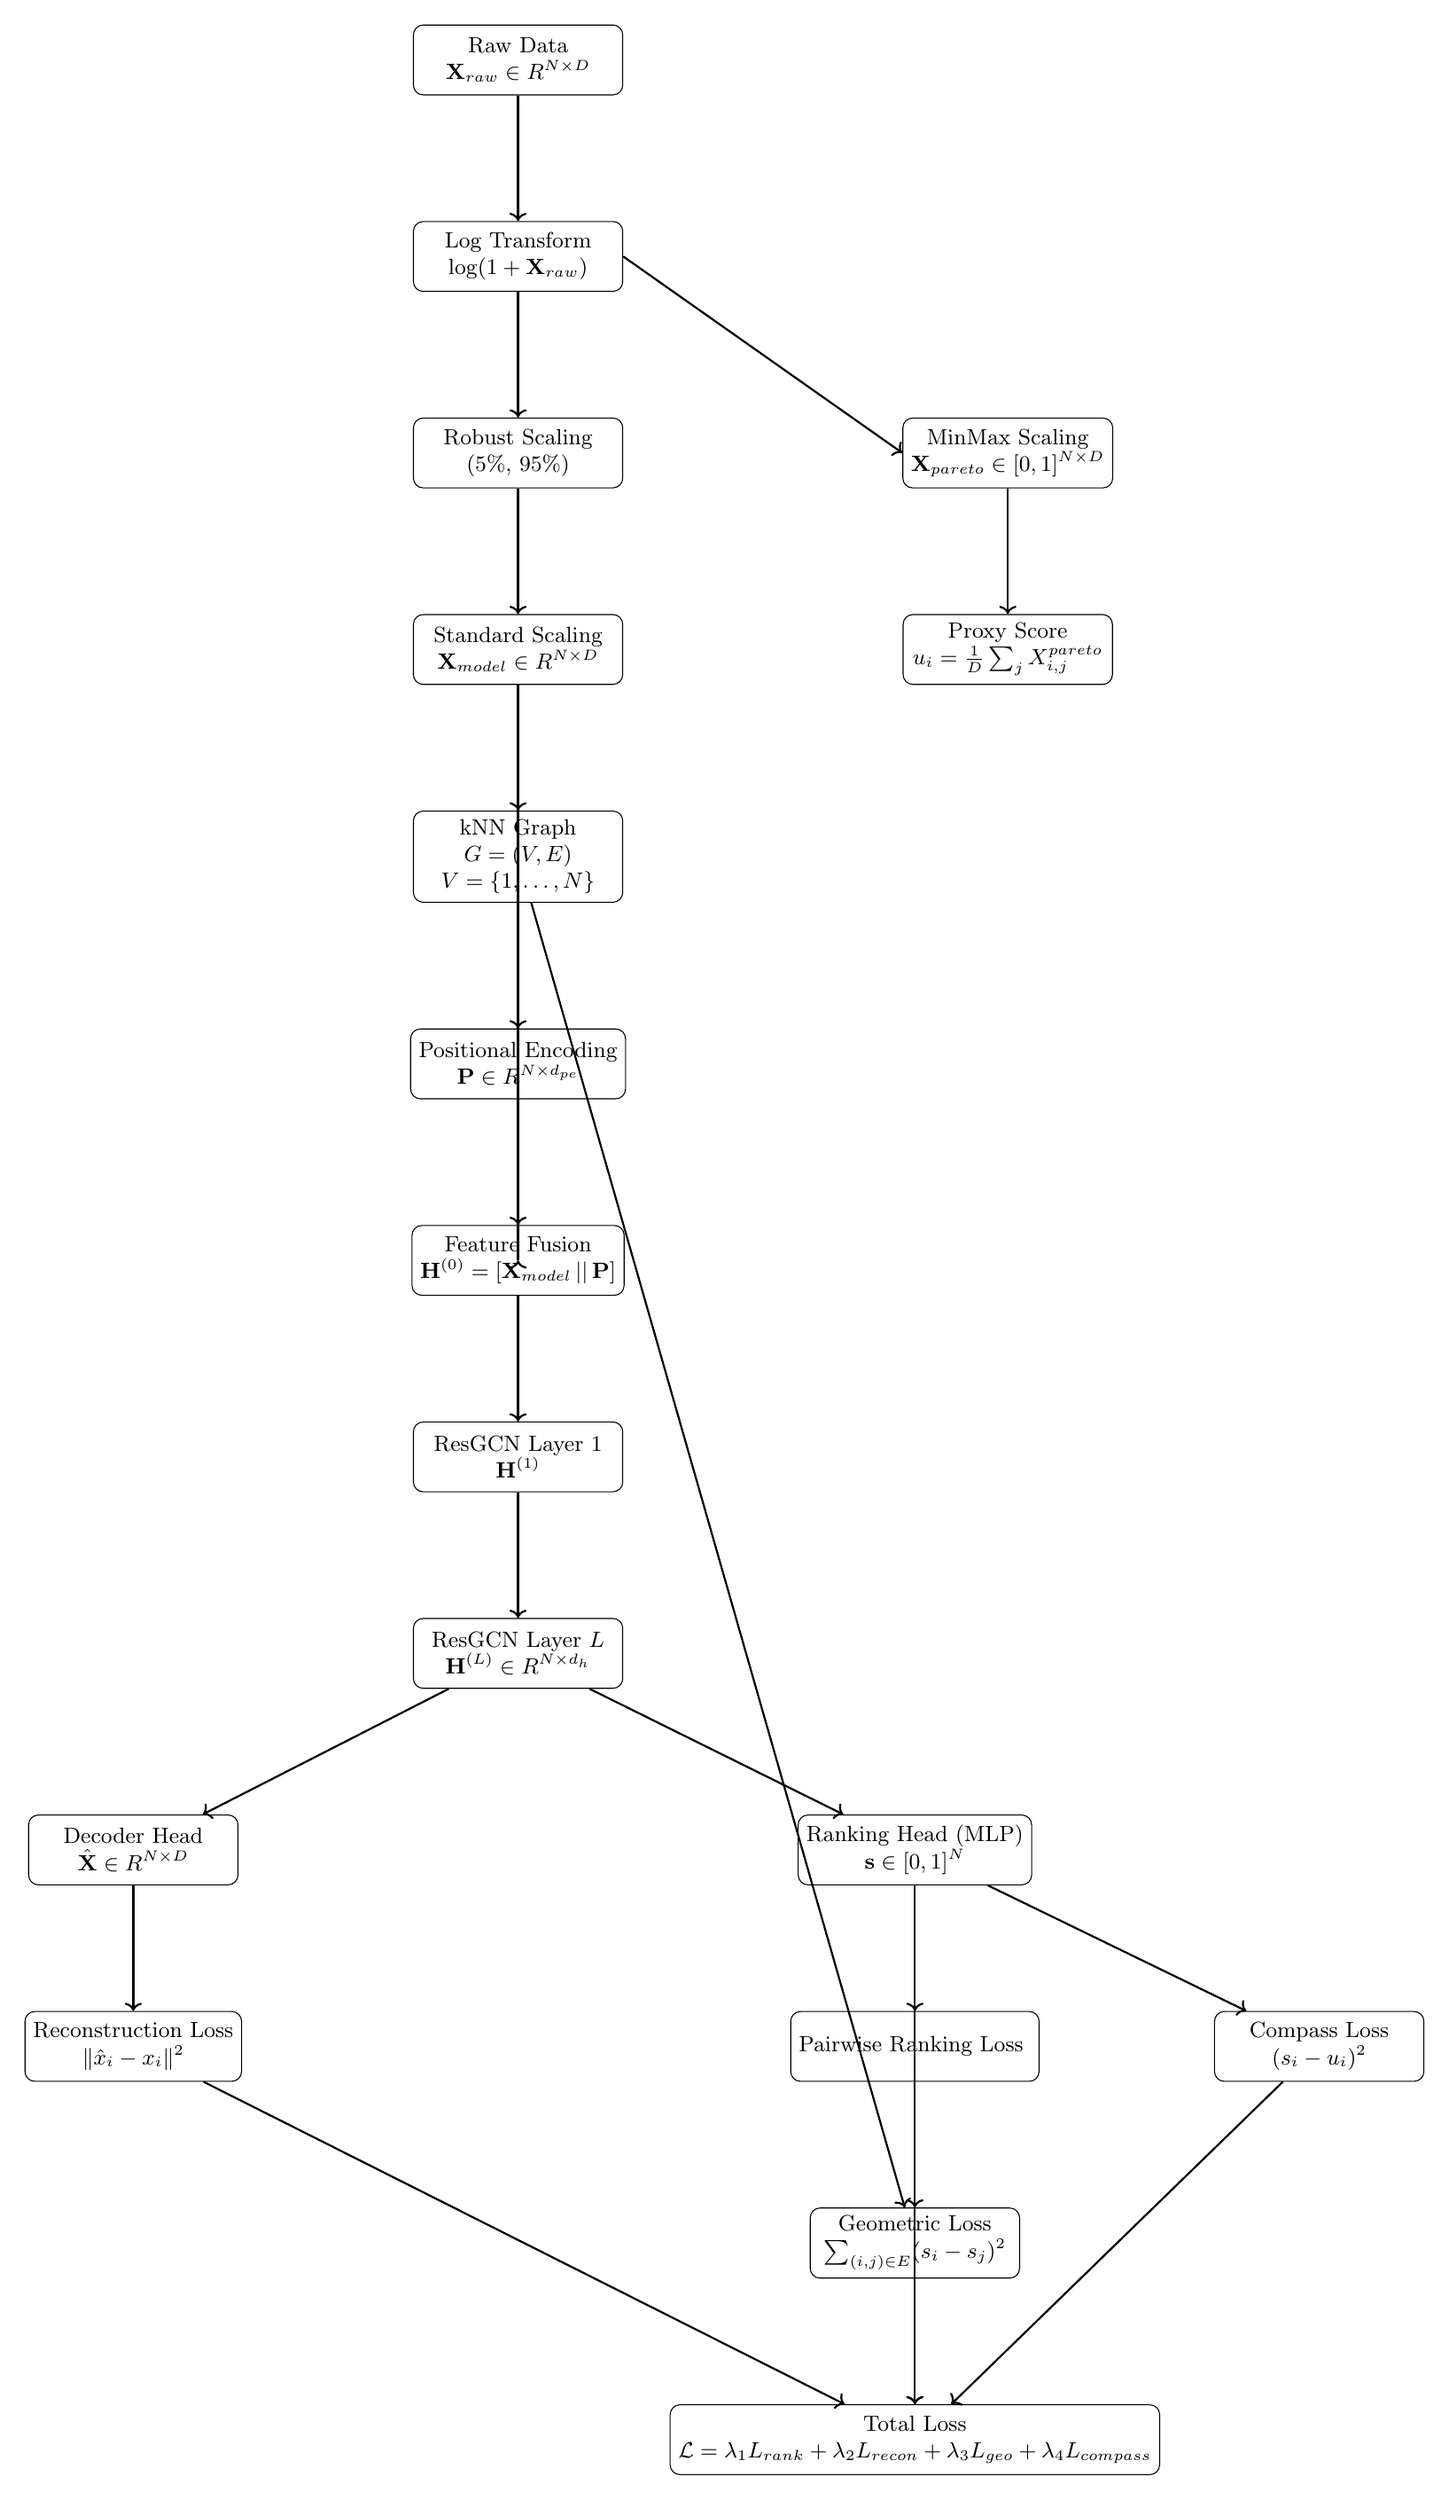
\begin{tikzpicture}[
    node distance=1.8cm and 2.5cm,
    every node/.style={font=\small},
    block/.style={rectangle, draw, rounded corners, align=center, minimum width=3cm, minimum height=1cm},
    arrow/.style={->, thick}
]

% INPUT
\node[block] (raw) {
Raw Data \\
$\mathbf{X}_{raw} \in \mathbb{R}^{N \times D}$
};

\node[block, below=of raw] (log) {
Log Transform \\
$\log(1 + \mathbf{X}_{raw})$
};

\node[block, below=of log] (robust) {
Robust Scaling \\
(5\%, 95\%)
};

\node[block, below=of robust] (std) {
Standard Scaling \\
$\mathbf{X}_{model} \in \mathbb{R}^{N \times D}$
};

\node[block, right=4cm of robust] (minmax) {
MinMax Scaling \\
$\mathbf{X}_{pareto} \in [0,1]^{N \times D}$
};

\node[block, below=of minmax] (proxy) {
Proxy Score \\
$u_i = \frac{1}{D} \sum_j X^{pareto}_{i,j}$
};

% GRAPH
\node[block, below=of std] (knn) {
kNN Graph \\
$G = (V,E)$ \\
$V = \{1,\dots,N\}$
};

\node[block, below=of knn] (posenc) {
Positional Encoding \\
$\mathbf{P} \in \mathbb{R}^{N \times d_{pe}}$
};

\node[block, below=of posenc] (concat) {
Feature Fusion \\
$\mathbf{H}^{(0)} = [\mathbf{X}_{model} \, || \, \mathbf{P}]$
};

% GNN
\node[block, below=of concat] (gnn1) {
ResGCN Layer 1 \\
$\mathbf{H}^{(1)}$
};

\node[block, below=of gnn1] (gnn2) {
ResGCN Layer $L$ \\
$\mathbf{H}^{(L)} \in \mathbb{R}^{N \times d_h}$
};

% HEADS
\node[block, below left=of gnn2] (decoder) {
Decoder Head \\
$\hat{\mathbf{X}} \in \mathbb{R}^{N \times D}$
};

\node[block, below right=of gnn2] (ranker) {
Ranking Head (MLP) \\
$\mathbf{s} \in [0,1]^N$
};

% LOSSES
\node[block, below=of decoder] (reconloss) {
Reconstruction Loss \\
$\|\hat{x}_i - x_i\|^2$
};

\node[block, below=of ranker] (rankloss) {
Pairwise Ranking Loss
};

\node[block, right=of rankloss] (comploss) {
Compass Loss \\
$(s_i - u_i)^2$
};

\node[block, below=of rankloss] (geoloss) {
Geometric Loss \\
$\sum_{(i,j)\in E} (s_i - s_j)^2$
};

\node[block, below=of geoloss] (total) {
Total Loss \\
$\mathcal{L} = \lambda_1 L_{rank} + \lambda_2 L_{recon} + \lambda_3 L_{geo} + \lambda_4 L_{compass}$
};

% ARROWS
\draw[arrow] (raw) -- (log);
\draw[arrow] (log) -- (robust);
\draw[arrow] (robust) -- (std);
\draw[arrow] (log.east) -- (minmax.west);
\draw[arrow] (minmax) -- (proxy);

\draw[arrow] (std) -- (knn);
\draw[arrow] (knn) -- (posenc);
\draw[arrow] (posenc) -- (concat);

\draw[arrow] (std) |- (concat);
\draw[arrow] (concat) -- (gnn1);
\draw[arrow] (gnn1) -- (gnn2);

\draw[arrow] (gnn2) -- (decoder);
\draw[arrow] (gnn2) -- (ranker);

\draw[arrow] (decoder) -- (reconloss);
\draw[arrow] (ranker) -- (rankloss);
\draw[arrow] (ranker) -- (comploss);
\draw[arrow] (ranker) -- (geoloss);
\draw[arrow] (knn) -- (geoloss);

\draw[arrow] (reconloss) -- (total);
\draw[arrow] (rankloss) -- (total);
\draw[arrow] (comploss) -- (total);
\draw[arrow] (geoloss) -- (total);

\end{tikzpicture}

\end{document}